\documentclass[a4paper]{article}
\usepackage[letterpaper, margin=1in]{geometry} % page format
\usepackage{listings} % this package is for including code
\usepackage{graphicx} % this package is for including figures
\usepackage{amsmath}  % this package is for math and matrices
\usepackage{amsfonts} % this package is for math fonts
\usepackage{tikz} % for drawings
\usepackage{hyperref} % for urls
\usepackage{stackengine}

\title{Homework 0}
\author{Kaitlyn Mulligan}
\date{1/30/19}

\begin{document}
\lstset{language=Python}

\maketitle

\section{Python}
Below is the script I used to install the packages.\\
\lstinputlisting[language=Python,frame=single]{pythonInstall.py}
Here is the output of the print statements.\\
\begin{center}
  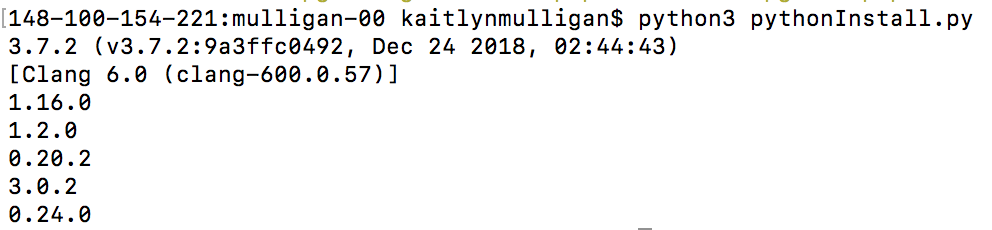
\includegraphics[width=1\textwidth]{output.jpg}
\end{center}

\section{GitHub}
My username on GitHub is \textbf{kmulligan48}.  The link to my repository is 
\textbf{https://github.com/kmulligan48/data440.git}.  Below is a screenshot to show that 
Professor Rivas has been added as a collaborator.
\begin{center}
  
\includegraphics[width=1\textwidth]{collaborator.jpg}
\end{center}

\section{Kaggle}
My Kaggle username is \textbf{kmulligan1} and below is a screenshot of my account.
\begin{center}
  
\includegraphics[width=1\textwidth]{kaggle.jpg}
\end{center}

\section{Problems}
\textbf{1.} For the function $g(x) = -3x^2 +24x -30$, find the value of $x$ that 
maximizes $g(x)$.\\

\textbf{Solution:} First we take the derivative of $g(x)$ which results in
\begin{equation*}
  g'(x) = -6x+24.
\end{equation*}

Next, set the derivative equal to zero and solve for $x$.  This results in $x=4$.  
To test to see if that is a maximum we can plug in a number less than and greater 
than $x=4$ to the derivative.  We can see that less than $4$, the derivative is positive 
and greater than $4$, the derivative is negative.  Therefore, $x=4$ is a value of $x$ 
that maximizes $g(x)$.\\
\textbf{2.} Consider the following function:
\begin{equation}
  f(x) = 3x_0^3 - 2x_0x_1^2 + 4x_1 - 8
\end{equation}
what are the partial derivatives of $f(x)$ with respect to $x_0$ and $x_1$.\\

\textbf{Solution:} The partial derivative of $f(x)$ with respect to $x_0$ is:
\begin{equation*}
  \frac{\partial f}{\partial x_0} = 9x_0^2-2x_1^2.
\end{equation*}

The partial derivative of $f(x)$ with respect to $x_1$ is:
\begin{equation*}
  \frac{\partial f}{\partial x_1} = -4x_0x_1+4.
\end{equation*}\\
\textbf{3.} Consider the matrix $A = 
\begin{bmatrix}
  1 & 4 & -3\\
  2 & -1 & 3
\end{bmatrix}$
and $B =
\begin{bmatrix}
  -2 & 0 & 5\\
  0 & -1 & 4
\end{bmatrix}$, then answer the following and verify your answers in Python:\\
\textbf{(a)} can you multiply the two matrices?  Ellaborate on your answer.\\

\textbf{Solution:} No, you cannot multiply these two matrices.  In order to multiply 
two matrices, the number of columns of the first matrix needs to equal the number of 
rows of the second matrix.  In this case, the number of columns in matrix A is 3, which 
does not equal the number of rows in matrix B which is 2.\\
Using Python to verify my answers, I ran the script below.
\lstinputlisting[language=Python,frame=single]{badMatrix.py}
This resulted in the following output which proves that we cannot multiply these two 
matrices.
\begin{center}
  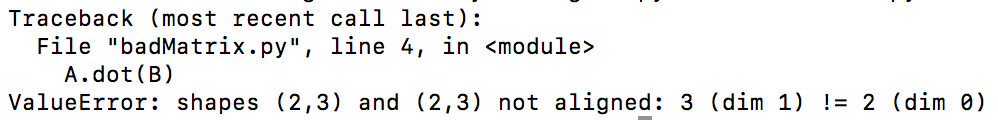
\includegraphics[width=1\textwidth]{badMatrix.jpg}
\end{center}
\textbf{(b)} multiply $A^T$ and B and give its \textit{rank}.\\

\textbf{Solution:}
We begin by finding the transpose of $A$ which is the following:
\begin{center}
  $A^T =
\begin{bmatrix}
  1 & 2\\
  4 & -1\\
  -3 & 3
\end{bmatrix}$.
\end{center}

Next we can multiply $A^T$ and $B$ as follows:
\begin{center}
$A^TB =
\begin{bmatrix}
  1 & 2\\
  4 & -1\\
  -3 & 3
\end{bmatrix}
\begin{bmatrix}
  -2 & 0 & 5\\
  0 & -1 & 4
\end{bmatrix}=
\begin{bmatrix}
  -2 & -2 & 13\\
  -8 & 1 & 16\\
  6 & -3 & -3
\end{bmatrix}$.
\end{center}
To find the rank, we need to reduce it to reduced row echelon form as follows:
\begin{center}
  $\begin{bmatrix}
    -2 & -2 & 13\\
    -8 & 1 & 16\\
    6 & -3 & -3
  \end{bmatrix}
  \to
  \begin{bmatrix}
    -2 & -2 & 13\\
    0 & 9 & -36\\
    0 & -9 & 36
  \end{bmatrix}
  \to
  \begin{bmatrix}
    1 & 1 & \frac{-13}{2}\\
    0 & 1 & -4\\
    0 & 0 & 0
  \end{bmatrix}
  \to
  \begin{bmatrix}
    1 & 0 & \frac{-5}{2}\\
    0 & 1 & -4\\
    0 & 0 & 0
  \end{bmatrix}$.
\end{center}
As we can see, there are two non-zero rows.  Therefore, the rank is 2.\\
Using Python to verify my answers, I ran the script below.\\
\lstinputlisting[language=Python,frame=single]{goodMatrix.py}
This resulted in the following output which verifies the answers I got.\\
\begin{center}
  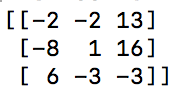
\includegraphics[width=0.18\textwidth]{goodMatrix.jpg}
\end{center}
\textbf{(c)} (extra credit) let $C =
\begin{bmatrix}
  1 & 0\\
  0 & 2
\end{bmatrix}$
be a new matrix; what is the result of $AB^T+C^{-1}$?\\

\textbf{Solution:} We begin by finding the transpose of B which is the following:
\begin{center}
  $B^T =
\begin{bmatrix}
  -2 & 0\\
  0 & -1\\
  5 & 4
\end{bmatrix}$.
\end{center}

Next we need to find the inverse of $C$ as follows:
\begin{center}
  $C^{-1} = \frac{1}{2}
\begin{bmatrix}
  2 & 0\\
  0 & 1
\end{bmatrix} =
\begin{bmatrix}
  1 & 0\\
  0 & \frac{1}{2}
\end{bmatrix}$.
\end{center}

Now we can solve $AB^T+C^{-1}$ as follows:
\begin{center}
  $AB^T+C^{-1} =
  \begin{bmatrix}
    1 & 4 & -3\\
    2 & -1 & 3
  \end{bmatrix}
  \begin{bmatrix}
    -2 & 0\\
    0 & -1\\
    5 & 4
  \end{bmatrix} +
  \begin{bmatrix}
    1 & 0\\
    0 & \frac{1}{2}
  \end{bmatrix} =
  \begin{bmatrix}
    -17 & -16\\
    11 & 13
  \end{bmatrix} +
  \begin{bmatrix}
    1 & 0\\
    0 & \frac{1}{2}
  \end{bmatrix} =
  \begin{bmatrix}
    -16 & -16\\
    11 & \frac{27}{2}
  \end{bmatrix}$.
\end{center}

Therefore, $AB^T+C^{-1} =
\begin{bmatrix}
  -16 & -16\\
  11 & \frac{27}{2}
\end{bmatrix}$.\\
Using Python to verify my answers, I ran the script below.
\lstinputlisting[language=Python,frame=single]{ECMatrix.py}
This resulted in the following output which verifies the answers I got.\\
\begin{center}
  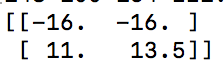
\includegraphics[width=0.18\textwidth]{ECMatrix.jpg}
\end{center}

\textbf{4.} Give the mathematical definitions of the simple Gaussian, multivariate 
Gaussian, Bernoulli, binomial, and exponential distributions.\\

\textbf{Solution:} \textbf{(a)} simple Gaussian distribution - otherwise known as the normal 
distribution, has a bell shaped curve, the pdf is given as $\frac{1}{\sigma \sqrt{2 
\pi}}e^{\frac{-(x-\mu)^2}{2\sigma^2}}$\\

\textbf{(b)} multivariate Gaussian distribution - otherwise known as multivariate normal 
distribution or joint normal distribution, it is a generalization of the one-dimensional 
normal distribution to a higher dimension, the pdf is given as $(2 \pi)^{\frac{-k}{2}}|\Sigma|
^{\frac{-1}{2}}e^{\frac{-1}{2}(x-\mu)^T \Sigma^{-1}(x-\mu)}$\\

\textbf{(c)} Bernoulli distribution - a discrete distribution having two possible outcomes labelled by 
$x=0$ or $x=1$ in which $x=1$ occurs with probability $p$ and $x=0$ occurs with probability 
$q=1-p$, where $0<p<1$, the pdf is given as $p^x(1-p)^{1-x}$\\

\textbf{(d)} binomial distribution - the discrete probability distribution, with parameters $n$ and $p$, 
of the number of successes in a sequence of $n$ independent experiments, the pdf is given as 
${n \choose x} p^x (1-p)^{n-x}$\\

\textbf{(e)} exponential distribution - the probability distribution that describes a process in which 
events occur continuously and independently at a constant average rate, the pdf is given as 
$\frac{1}{\beta}e^{\frac{-x}{\beta}}$\\
\textbf{5.} (extra credit) What is the relationship between the Bernoulli and binomial 
distributions?\\

\textbf{Solution:} The relationship between the Bernoulli and binomial distributions is that 
the Bernoulli distribution is a special case of the binomial distribution.  This is because a 
single trial is conducted.  This would mean $n$ is 1 for a binomial distribution.  In other words, 
a binomial random variable is a random variable that represents the number of successes in $n$ 
successive independent trials of a Bernoulli distribution.\\
\textbf{6.} Suppose that random variable $X \sim N(2, 3)$.  What is its expected value?\\

\textbf{Solution:} The expected value of $X \sim N(2, 3)$ is $2$.\\
\textbf{7.} An \textit{euclidean projection} of a $d$-dimensional point $y \in \mathbb{R}^d$ 
to a set $\mathcal{Z}$ is given by the following optimization problem:
\begin{equation}
  x^* = \mathop{\arg \min}_{x} ||x - y||^2_2 \text{, \space subject to: } x \in \mathcal{Z}
\end{equation}
where $\mathcal{Z}$ is the feasible set, $||\cdot||_2$ is the $\ell_2$-norm (euclidean) of a 
vector, and $x^* \in \mathbb{R}^d$ is the projected vector.\\
\textbf{(a)} What is $x^*$ if $y=1.1$ and $\mathcal{Z} = \mathbb{N}$, where $\mathbb{N}$ is the 
set of natural numbers?\\

\textbf{Solution:} We know that $y=1.1$ and $\mathcal{Z} = \mathbb{N}$.  To figure out what $x^*$ 
is, I will plug in some natural numbers starting at $1$ and increasing to see which values of $x^*$ 
minimize the given optimization problem. First plugging $1$ in, we see that the distance between 
these points is $\sqrt{(1-1.1)^2} = \sqrt{(-0.1)^2} = \sqrt{0.01} = 0.1$.  Next plugging in $2$, 
the distance is $\sqrt{(2-1.1)^2} = \sqrt{(0.9)^2} = \sqrt{0.81} = 0.9$.  Continuing to see the 
pattern, plugging in $3$, the distance is $\sqrt{(3-1.1)^2} = \sqrt{(1.9)^2} = \sqrt{3.61} = 1.9$.  
The natural numbers we are plugging in are continuously increasing and the results we are obtaining 
are also continuously increasing.  Therefore, the first value we plugged in, $1$, is the value of 
$x^*$ that will minimize this optimization problem given.  The smallest result we obtain is $0.1$, 
therefore $x^* = 1$.\\
\textbf{(b)} Locate $x^*$ in the following picture:
\begin{center}
  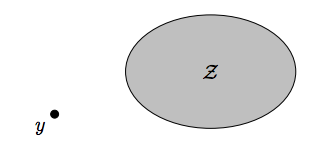
\includegraphics[width=0.3\textwidth]{question7.jpg}
\end{center}

\textbf{Solution:} In this picture, $x^*$ is located at the red dot.
\begin{center}
  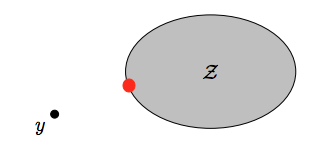
\includegraphics[width=0.3\textwidth]{question7solution.jpg}
\end{center}
\textbf{8.} Suppose that random variable Y has distribution:
\[
  p(Y=y) =
  \begin{cases}
  e^{-y} & \text{if } y \geq 0\\
  0 & \text{otherwise}
  \end{cases}
\]
\textbf{(a)} Verify that $\int_{y=-\infty}^\infty p(Y=y) = 1$.

\textbf{Solution:} To verify this integral we have:
\begin{align*}
\int_{y=-\infty}^\infty p(Y=y) &= \int_{-\infty}^0 p(Y=y) + \int_{0}^\infty p(Y=y)\\
&= \int_{-\infty}^0 0 + \int_{0}^\infty e^{-y}\\
&= 0 + \int_{0}^\infty e^{-y}\\
&= -e^{-y} \Big|_0^\infty\\
&= -e^{-\infty} - (-e^{-(0)})\\
&= 0 + 1\\
&= 1.
\end{align*}

Thus we have shown that $\int_{y=-\infty}^\infty p(Y=y) = 1$.\\
\textbf{(b)} What is $\mu_Y = E[Y] = \int_{y=-\infty}^\infty p(Y=y) y dy$; that is, the expected 
value of $Y$?

\textbf{Solution:} To find $\mu_Y$ we have:
\begin{align*}
  \mu_Y &= E[Y]\\
  &= \int_{y=-\infty}^\infty p(Y=y) y dy\\
  &= \int_{-\infty}^0 p(Y=y) y dy + \int_{0}^\infty p(Y=y) y dy\\
  &= \int_{-\infty}^0 (0)(y) dy + \int_{0}^\infty (e^{-y}) (y) dy\\
  &= \int_{-\infty}^0 0 dy + \int_{0}^\infty ye^{-y} dy\\
  &= 0 + \int_{0}^\infty ye^{-y} dy\\
  &= \int_{0}^\infty ye^{-y} dy.
\end{align*}

Using integration by parts and our previous solution, we can solve this integral as follows:
\begin{align*}
  \mu_Y &= \int_{0}^\infty ye^{-y} dy\\
  &= -ye^{-y} \Big|_0^\infty + \int_0^\infty e^{-y} dy\\
  &= -ye^{-y} - e^{-y} \Big|_0^\infty\\
  &= e^{-y} (-y-1) \Big|_0^\infty\\
  &= [e^{-\infty} (-\infty-1)] - [e^{-(0)} (-(0)-1)]\\
  &= 0 - [1 (-1)]\\
  &= 1.
\end{align*}

Thus we have $\mu_Y = 1$.\\
\textbf{(c)} What is $\sigma^2 = \text{Var}[Y] = \int_{y=-\infty}^\infty p(Y=y) (y - \mu_Y)^2 dy$;
that is, the variance of Y?

\textbf{Solution:} To find $\sigma^2$ we have:
\begin{align*}
  \sigma^2 &= \text{Var}[Y]\\
  &= \int_{y=-\infty}^\infty p(Y=y) (y - \mu_Y)^2 dy\\
  &= \int_{-\infty}^0 p(Y=y) (y - \mu_Y)^2 dy + \int_{0}^\infty p(Y=y) (y - \mu_Y)^2 dy\\
  &= \int_{-\infty}^0 (0) (y - \mu_Y)^2 dy + \int_{0}^\infty (e^{-y}) (y - \mu_Y)^2 dy\\
  &= 0 + \int_{0}^\infty (e^{-y}) (y - \mu_Y)^2 dy\\
  &= \int_{0}^\infty (e^{-y}) (y - \mu_Y)^2 dy.
\end{align*}

In the previous part we found that $\mu_Y = 1$, so now we can plug that into our integral as follows:
\begin{align*}
  \sigma^2 &= \int_{0}^\infty (e^{-y}) (y - \mu_Y)^2 dy\\
  &= \int_{0}^\infty (e^{-y}) (y - 1)^2 dy\\
  &= \int_{0}^\infty (e^{-y}) (y^2 -2y + 1) dy\\
  &= \int_{0}^\infty y^2e^{-y} -2ye^{-y} + e^{-y} dy\\
  &= \int_{0}^\infty y^2e^{-y}dy + \int_{0}^\infty-2ye^{-y}dy + \int_{0}^\infty e^{-y} dy\\
  &= \int_{0}^\infty y^2e^{-y}dy -2 \int_{0}^\infty ye^{-y}dy + \int_{0}^\infty e^{-y} dy.
\end{align*}

Using parts a and b, we can plug our results into the second two integrals we have.  For the first integral, we can 
solve it using integration by parts as follows:
\begin{align*}
  \sigma^2 &= \int_{0}^\infty y^2e^{-y}dy -2 \int_{0}^\infty ye^{-y}dy + \int_{0}^\infty e^{-y} dy\\
  &= \left(-y^2e^{-y} \Big|_0^\infty + 2\int_{0}^\infty ye^{-y}dy \right) -2 \left(e^{-y} (-y-1) \Big|_0^\infty \right) + \left(-e^{-y} \Big|_0^\infty\right)\\
  &= \left((0 - 0) + 2 (e^{-y} (-y-1) \Big|_0^\infty \right) -2 (1) + 1\\
  &= 2(1) -2(1) + 1\\
  &= 2 - 2 + 1\\
  &= 1.
\end{align*}

Therefore we have $\sigma^2 = 1$.\\
\textbf{(d)} What is $E[Y | Y \geq 10]$; that is, the expected value of $Y$, given that (or conditioned 
on) $Y \geq 10$?

\textbf{Solution:} To find $E[Y | Y \geq 10]$ we have:
\begin{align*}
  E[Y | Y \geq 10] &= \int_{10}^\infty p(Y=y) y dy\\
  &= \int_{10}^\infty (e^{-y})(y) dy\\
  &= \int_{10}^\infty ye^{-y} dy.
\end{align*}

From here we can use our results from above to find:
\begin{align*}
  E[Y | Y \geq 10] &= \int_{10}^\infty ye^{-y} dy\\
  &= e^{-y} (-y-1) \Big|_{10}^\infty\\
  &= [e^{-\infty} (-\infty-1)] - [e^{-10} (-10-1)]\\
  &= 0 - [e^{-10} (-11)]\\
  &= 11e^{-10}.
\end{align*}

Therefore, we have $E[Y | Y \geq 10] = 11e^{-10}$.

\end{document}
